\chapter{Neighbourhood component analysis}
\label{ch:nca}

	Neighbourhood component analysis (NCA; \citealp{goldberger2004}) is another
	method that has the goal of learning a Mahalobnis-like metric. It was developed
	with $k$NN in mind; from a practical point of view NCA can be viewed as a
	recommended additional step when doing classification with $k$NN. 

\section{General presentation}
\label{sec:general-presentation}

	Because the goal is to enhance the $k$NN performance, the first idea the authors
	had was to maximize the leave one out cross validation performance: we take each 
	point in the data set and try to classify it using $k$NN. Unfortunately, there does
	not exist an exact correlation between the linear transformation $\AB$ and the nearest neighbours
	for a given point: a small perturbation of $\AB$ might cause strong changes or, conversely, 
	it might leave the neighbours unchanged. This means that any function of the neighbours
	is piecewise constant and discontinuous and, hence, hard to optimize.
	
	So they proposed a function that behave better by introducing the concept of stochastic nearest
	neighbours. These are achieved by adding randomization to the classification process. In the classical case, the query point gets the label of the closest point. In the stochastic nearest neighbour 
	case, the query point inherits the label of a neighbour with a probability that is inverse proportional with the distance. They used a function a probability function that is reminiscent to the softmax activation used for neural network or to the generalized logistic function.
	
	The probability that the point $j$ is selected the nearest neighbour of the point $i$ is given by:
	\begin{align}
		p_{ij} = \frac{
						\exp(-d_{ij}^2)
					  }{
						\sum_{\substack{k=1 \\k\neq i}}^N\exp(-d_{ik}^2)
					  }
	\label{eq:stochastic-neighbour}
	\end{align}
	
	Also we have to define that $p_{ii}=0$: point $i$ cannot pick itself as the nearest neighbour.
	Note that these stochastic assignment are function of the distances and implicitly, they are depend on the point positions. Because the point position change with the linear transformation $\AB$, it means that $p_{ij}$ are function of $\AB$ and, furthermore, $p_{ij}$ are differentiable with respect to $\AB$.
	
	Because we want to improve the classification accuracy, we want to maximize the probability of our point $i$ of being selected by points that belong to its true class (equivalently, the probability of the point of being correctly classified). This quantity is denoted by $p_i$:
	\begin{align}
		p_i = \sum_{j\in c_i} p_{ij}.
	\end{align}
	
	By considering each point and the probability of belonging to its true class, we get the objective function:
	\begin{align}
		f(\AB) &= \sum_{i=1}^N p_i\\
			   &= \sum_{i=1}^N \sum_{j\in c_i} \frac{
								\exp(-d_{ij}^2)
							  }{
								\sum_{k\neq i}\exp(-d_{ik}^2)
							  }.
	\end{align}
	
	This can also be interpreted as the expected number of the correctly classified points.
	
	By differentiating with respect to $A$, we obtain the gradient:
	\begin{align}
	  \frac{\partial f}{\partial
	A}=2A\sum_{i=1}^{N}\left(p_i\sum_{k=1}^Np_{ik}\xB_{ik}\xB_{ik}^{\textrm{T}} -
	\sum_{j\in c_i}p_{ij}\xB_{ij}\xB_{ij}^{\textrm{T}} \right)\label{eq:nca-grad},
	\end{align}
	where $\xB_{ij} = \xB_i - \xB_j$.
	
	The derivation of the gradient can be found in the appendix. The gradient offers us the possibility of optimizing the function using a gradient based solver.
	
	NCA does not assume anything about the classes structure, permits very diverse metrics. It comes at some cost: the objective function is not convex. There appear some problems like initialization and optimization which are treated more in detail in Section \ref{sec:practical-notes}. Another problem is the computational cost. For each point we need to compute all the distances to other points. This scales in $N^2$ which is intractable for large data sets. Actually, the a function evaluation is in $\mathcal{O}(dDN^2)$. Chapter \ref{ch:reducing} presents various solutions to mitigate this problem.
	
	The general scenario in which NCA is applied can be described by the training and testing steps:
	describe algorithm.
	%\begin{itemize}
	%   \item
	%\end{itemize}
	
\section{Class-conditional kernel density estimation interpretation}
\label{sec:cc-kde}
	
	\begin{figure}
	  \centering
	  \subfigure[Illustration of the class as a mixture of
	Gaussians.]{\label{fig:mog}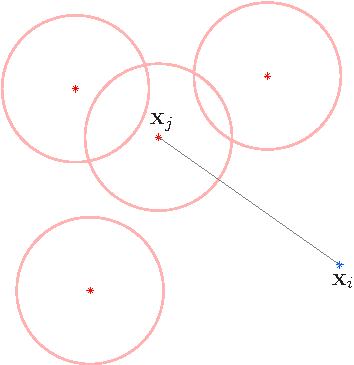
\includegraphics[width=6cm]{images/mog}}
	%\subfigure[The projection $\AB$ applied to the whole data set
	%$\mathcal{D}$.]{\label{fig:sub-sampling-2}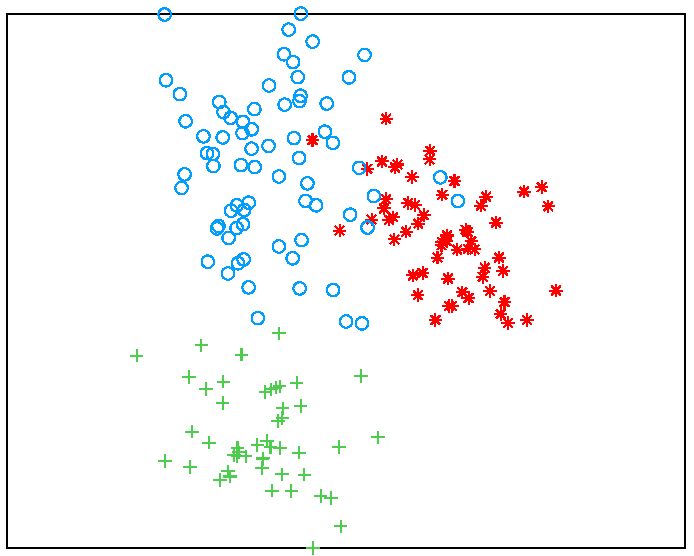
\includegraphics[width=0.48\textwidth]{images/sub-sample-2}}
	  \caption{Formulating NCA as a class-conditional kernel density estimation
	framework.}
	  \label{fig:kde}
	\end{figure}
	
	In this section we will present NCA into a class-conditional kernel density
	estimation framework. This interpretation will allow us to understand what are
	the assumptions behind NCA. Moreover, this also offers the possibility of
	altering the model in a suitable way that is efficient for computations. We will
	see this in the sections \ref{sec:approximate} and \ref{sec:exact-computations}.
	Similar ideas were previously presented by and , but the following were derived
	independently and they offer different insights. The following interpretation
	was inspired by the probabilistic $k$NN presented by \citet{barber2011}.
	
	We start with the basic assumption that each class can be modelled by a mixture
	of Gaussians. For each of the $N_c$ data points in class $c$ we consider a
	Gaussian ``bump'' centred around it. From a generative perspective, we can view
	that each point $\xB_j$ can generate a point $\xB_i$ with a probability given by
	an isotropic normal distribution with variance $\sigma^2$:
	\begin{align}
	    p(\xB_i|\xB_j) &= \mathcal{N}(\xB_i|\xB_j, \sigma^2\mathrm{I}_D) \\
	                   &= \frac{1}{(2\pi)^{D/2}}\exp \left\{-\frac{1}{2\sigma^2}
	(\xB_i - \xB_j)^\mathrm{T}(\xB_i - \xB_j)\right\}.
	\end{align}
	
	By changing the position of the points through a linear transformation $\AB$,
	the probability changes as follows:
	\begin{align}
	    p(\AB\xB_i|\AB\xB_j) \propto \exp \left\{-\frac{1}{2\sigma^2} (\xB_i -
	\xB_j)^\mathrm{T}\AB^\mathrm{T}\AB(\xB_i - \xB_j)\right\}.
	\end{align}
	
	We can note that this is similar to the $p_{ij}$ from NCA. Both
	$p(\AB\xB_i|\AB\xB_j)$ and $p_{ij}$ are directly proportional with the same
	quantity.
	
	Using the mixture of Gaussians assumption, we have that the probability of a
	point of being generated by class $c$ is equal to the sum of all Gaussians in
	class $c$:
	\begin{align}
	    p(\xB_i|c) &= \frac{1}{N_c}\sum_{\xB_j \in c} p(\xB_i|\xB_j)\\
	               &= \frac{1}{N_c}\sum_{\xB_j \in c} \mathcal{N}(\xB_i|\xB_j,
	\mathrm{I}_D).
	\end{align}
	
	However, we are interested on the inverse probability, given a point $\xB_i$
	what is the probability of $\xB_i$ belonging to class $c$. We can obtain an
	expression for $p(c|\xB_i)$ using Bayes' theorem:
	\begin{align}
	    p(c|\xB_i) = \frac{p(\xB_i|c)p(c)}{p(c|\xB_i)} =
	\frac{p(\xB_i|c)p(c)}{\sum_{c} p(\xB_i|c)p(c)}.
	    \label{eq:nca-cc-kde-bayes}
	\end{align}
	
	Now if further consider the classes to be equal probable (which might a
	reasonable assumption if we have no a priori information) we arrive at result
	that resembles the expression of $p_i$ (see equation):
	\begin{align}
	%   &p(c|\xB_i) = \frac{p(\xB_i|c)}{\sum_{c} p(\xB_i|c)}\\
	    p(c|\AB\xB_i) = \frac{
	                \frac{1}{N_c}\sum_{\xB_j \in
	c}\exp\left\{-\frac{1}{2\sigma^2}(\xB_i -
	\xB_j)^\mathrm{T}\AB^\mathrm{T}\AB(\xB_i - \xB_j)\right\}
	                }
	                {
	                \frac{1}{N_{c'}}\sum_{c'} \sum_{\xB_k \in
	c'}\exp\left\{-\frac{1}{2\sigma^2}(\xB_i -
	\xB_k)^\mathrm{T}\AB^\mathrm{T}\AB(\xB_i - \xB_k)\right\}
	                }
	\end{align}
	
	%In the numerator we have the sum of
	We are interested in predicting the correct class of the point $\xB_i$. So we
	try to find that linear transformation $\AB$ that maximises the class
	conditional probability of this point $p(c_i|\xB_i)$ to its true class $c_i$.
	\begin{align}
	    f(\AB) = \sum_i p(c_i|\AB\xB_i).
	    \label{eq:nca-cc-kde-obj}
	\end{align}.
	
	The gradient of the objective function is the following:
	\begin{align}
	    \frac{\partial f}{\partial \AB} =
	      \sum_i \left\{
	                \frac
	                {
	                    \frac{\partial p(\AB\xB_i|c)}{\partial \AB}p(c)
	                }
	                {
	                    \sum_c p(\xB_i|c)p(c)
	                }
	                - \underbrace{\frac{
	                    p(\AB\xB_i|c)p(c)
	                }{
	                    \sum_c p(\AB\xB_i|c)p(c)
	                }}_{p(c|\AB\xB_i)}
	                \frac{
	                    \sum_c \frac{\partial p(\AB\xB_i|c)}{\partial \AB}p(c)
	                }{
	                    \sum_c p(\AB\xB_i|c)p(c)
	                }
	             \right \}.
	    \label{eq:nca-cc-kde-grad}
	\end{align}
	

\section{Practical notes}
\label{sec:practical-notes}

	This section provides some practical advice for the questions 
	that can be raised while implementing NCA. 
	While NCA is not that hard to implement, there is needed certain care
	in order to achieve good solutions.

\subsection{Optimization methods}
\label{subsec:optimization}

\begin{itemize}
    \item We have the first-order gradient information; so, we
        can use any gradient based method.
    \item Gradient descent is an iterative algorithm that uses
        first-order information to find a minimum of a
        function. At each step, it proposes to go in the
        steepest direction, \ie, the direction with largest
        gradient. It is a very simple to implement method, but
        suffers from known convergence drawbacks. For example,
        there might appear the zig-zagging effect it depends
        on some critical parameters which make it difficult to
        use in practice. These are the learning rate $\eta$
        and the convergence conditions.
    \item Common choices for $\eta$ are either using a
        constant step or decrease it gradually. Using a
        constant step size can make the algorithm diverge.
    \item There are different other heuristics that make this
        more efficient. One of these is the bold-driver trick.
    \item A learning rate decreasing procedure is to set
        $\eta=\frac{\eta_0}{t + t_0}$, where $t$ represents
        the iteration number, $\eta_0$ and $t_0$ are
        constants. So, we end up with two hyper-parameters
        instead of one. There are various trick of tuning
        them. Leon Bottou mentions that a common value for
        $\eta_0$ is to be equal to the regularization variable
        and $t_0$ should then be selected such that the
        updates . In our implementation, because we did not
        use a regularization term, we set $\eta_0$ to a fix
        value and then we did an exponential search for $t_0$.
    \item One might also try to use momentum. For further
        useful advice on optimization one should consult
        BackProp.
    \item An improved version of the gradient descent is the
        conjugate gradients algorithm. This has better
        convergence.
\end{itemize}

\subsection{Initialization}
\label{subsec:initialization}

\begin{itemize}
    \item Important, because the function is not convex; we
        obtain different final solutions by using different
        starting points. In general, it is good idea to try
        multiple initial seeds and then select that $\AB$ that
        achieved the highest score.
    \item The simplest solution is to randomly choose values
        for the projection matrix $\AB$. We also tried to
        initialize with other linear transformations whose
        computational cost is cheap compared to NCA: principal
        component analysis (PCA; \citealp{pearson1901}),
        linear discriminant analysis (LDA;
        \citealp{fisher1936}) and relevant component analysis
        (RCA; \citealp{bar2003}).
    \item For completeness, we give the equations and further notes for these
methods here:
        \begin{itemize}
            \item  PCA finds an orthogonal linear
                transformation of the data. This is
                obtained by computing the
                eigendecomposition of the outer covariance
                matrix:
                \begin{align}
                    \SB = \frac{1}{N}\sum_{i=1}^N (\xB-\muB)(\xB-\muB)\tr.
                    \label{eq:pca-1}
                \end{align}

            \item LDA finds a linear transformation $\AB$ by maximizing the
variance between classes $\SB_B$ relative to the amount of within-class variance
$\SB_W$:
            \begin{align}
             \SB_B &=
\frac{1}{C}\sum_{c=1}^{C}\boldsymbol\mu_c\boldsymbol\mu_c\tr\label{eq:lda-1}\\
             \SB_W &= \frac{1}{N}\sum_{c=1}^{C}\sum_{i \in
c}(\mathbf{x}_i-\boldsymbol{\muB}_c)(\mathbf{x}_i-\boldsymbol{\mu}_c)\tr.\label{eq:lda-2}
            \end{align}

            The projection matrix $\AB$ that achieves this maximization consists
of the eigenvectors of $\SB_W^{-1}\SB_B$.

            We note that, unlike PCA, LDA makes use of the class labels and this
usually guarantees a better initial projection.

            \item RCA finds a linear transformation $\AB$
                that ``whitens'' the data with respect to
                the within-chunklet covariance matrix.
                Because for NCA we restrict ourselves to
                fully labelled data, the within-chunklet
                covariance is the within-class covariance
                $\SB_W$, Equation \ref{eq:lda-2}. The
                whitening transformation is then
                $\AB=\SB_W^{-1/2}$.
        \end{itemize}

        The methods above can be used for low-rank
        initialization as well: select only the top $d$ most
        discriminative eigenvectors, \ie, those that have the
        highest eigenvalues associated.

        From our experiments, we can conclude that a good
        initialization reflects in a good solution. For small
        and simple data sets this is not that obvious, but for
        large data sets the differences are more pregnant.
\end{itemize}

\subsection{Numerical issues}
\label{subsec:numerical-issues}

\begin{itemize}
    \item There are situations when we end up in the
        undetermined case $\frac{0}{0}$ while computing the
        soft assignments $p_i$. This happens when the point
        $\xB_i$ is far away from the rest of the points such
        that $p_{ij}$ is 0 in numerical precision. To make an
        idea of how big the distance between two points need
        to be such the contribution is zero, we give the
        example for \textsc{Matlab}: if \texttt{d>30} then
        \texttt{exp(-d\^{}2)=0}
    \item Unfortunately, this happens often in practice. The
        most obvious case is when we are dealing with
        outliers. But there are also other scenarios. The
        scale of the axes can be large and the linear
        projection $\AB$ cannot compensate for this. In this
        situation, we end up with almost all the points having
        this problem. This can also happen during training: a
        point might get ``thrown away'' during an update of
        $\AB$.
    \item A simple way to alleviate this is by normalizing the
        data, \ie, centering and making it unit variance:
        \begin{align}
            x_{ij} \leftarrow \frac{x_{ij} - \mu_j}{\sigma_j}, i =
\{1,\cdots,N\}, j = \{1,\cdots,D\}.
        \end{align}
        In this case we have to store these characteristics
        and then apply them on the test data. The total
        projection will the combination of two successive
        linear transformations:
        \begin{align}
            \AB \leftarrow \AB_{\text{learnt}}  \cdot \begin{pmatrix}
                  \sigma_1 &  \cdots & 0 \\
                  \vdots  &   \ddots & \vdots  \\
                  0 & \cdots & \sigma_D
                 \end{pmatrix}.
        \end{align}
    \item Because this does not guarantee the lack of
        numerical problem, we further corrected this issue by
        replacing each \texttt{NaN} with a very small value.
        This was inspired by Laurens van der Maaten
        implementation and we made use of it due to its
        simplicity. A more rigorous way of dealing with this
        would be by using the log-sum-exp trick. This idea is
        presented in detail in the appendix.

\end{itemize}

\subsection{Regularization}
\label{subsec:regularization}

\begin{itemize}
    \item NCA favours 1NN and large scale linear projections
        $\AB$. This is not usually the optimal thing.
    \item We can correct this using regularization, as pointed
        out in \citep{singh2010}.
        \begin{align}
            g(\AB) = f(\AB) - \lambda \sum_{i=1}^d\sum_{j=1}^D A_{ij}^2.\\
            \frac{\partial g}{\partial \AB} = \frac{\partial f}{\partial \AB} -
2\lambda\AB.
        \end{align}
    \item On the other hand, it is not clear how to set the
        regularization parameter $\lambda$ and how to choose
        the number of nearest neighbours for classification.
\end{itemize}

\subsection{Doing classification}
\label{subsec:doing-classification}

\begin{itemize}
    \item We optimize the objective function
        \ref{eq:nca-cc-kde-obj}. We found that for large data
        sets it is better to do classification using the
        probabilistic based approach: given a query point
        $\xB^*$ we assign to the most probable class $c =
        \operatorname{argmax}_cp(c|\xB^*)$.
\end{itemize}

\subsection{Dimensionality annealing}
\label{subsec:dimensionality-annealing}

\begin{itemize}
    \item
    \begin{align}
            g(\AB) = f(\AB) - \sum_{i=1}^D\lambda_i\sum_{j=1}^D A_{ij}^2.\\
            \frac{\partial g}{\partial \AB} = \frac{\partial f}{\partial \AB} - 2\begin{pmatrix}
                              \lambda_1A_{11} &  \cdots & \lambda_1A_{1D} \\
                              \vdots  &   \ddots & \vdots  \\
                              \lambda_dA_{d1} & \cdots & \lambda_dA_{dD}
                             \end{pmatrix}.
        \end{align}
\end{itemize}